\section{Renormalization Theory}
\begin{figure}[b]
\begin{center}
\includegraphics[scale=0.2]{fig/ising.png}
\caption{Studying a problem at multiple scales}
\label{fig:scales}
\end{center}
\end{figure}
The heart of our method for solving the TSP problem is the renormalization theory. The renormalization theory is originating from theoretical physics. In theoretical physics renormalization is used to study the observe the changes in a physical system. The changes are observed by looking to the problem at different scales. This idea is illustrated in figure \ref{fig:scales}.
\newline\newline\noindent
This idea is mapped onto the Traveling Salesman problem. The total square in figure \ref{fig:scales} can be seen as the total area where the cities are located. When estimating the shortest route, we start at a large scale, and we keep zooming in until our estimated path visiting all cities is known. The procedure is illustrated in figure \ref{fig:renormalization}. The image on the top left of the figure is the basic block. This basic block consists of four cells. A cell represents a virtual city, available if one or more cities are within the cell. The general idea of the algorithm is to solve the Traveling Salesman problem for the larger block. This can be done easily, because a Traveling Salesman problem for at most four cities can be easily solved, by simply enumerating all possibilities. Then this block can be divided into four subblocks. Together with some information acquired from the larger block, the Traveling Salesman problem can again be solved for the four subblocks. This process is repeated until there is at most one city in a cell, and the estimated route is known. In the following subsection we will describes the steps in the algorithm in more detail.
\subsection{Preprocessing step}
\begin{figure}[t]
\begin{center}
\includegraphics[scale=0.25]{fig/renormalization.pdf}
\caption{The basic two by two cell. The open circles are the border points, the closed circles are the centra of the cells and the crosses are additional places where an edge crosses the border of a cell}
\label{fig:renormalization}
\end{center}
\end{figure}
The preprocessing step prevents the performance penalty each time you need to calculate an optimal route in a block. Basically this means that for every possible configuration you calculate the optimal path. There are two aspects which can be altered, the border point at which the route is started and the visited cells.
\newline\newline\noindent
For retrieving the shortest route through a block, it is considered as a graph. The nodes are the border points and the cell points (Lying in the centrum of a cell). The nodes are connected by multiple
Before treating on the algorithm the preprocessing is considered.  The preprocessing consists of calculating all shortest paths in the basic blocks. Here all possible subsets of cells that needs to be visited are considered.
\newline\newline\noindent
The basic block can be treated as a graph, the border points and the cell points are the nodes. There are edges between the border points and their closest cell point(s). The cell points are also connected with an edge with the other cell points. This set-up can be seen in the top left picture of figure \ref{fig:renormalization}. For getting the shortest route, a breadth first search is used. Here all possible paths, without cycles, between the starting and end node are calculated. Using these set of paths, the shortest routes visiting subsets of cell points are searched.
\subsection{First iteration}
In the first iteration we start with one block with four cells. In such a block a subset of at least 3 cells needs to be occupied to form a starting tour. The cells where at least one city is located, are connected to form a shortest tour. This tour is an easy connection of the cities, an all the possible routes, do not need to be investigated.
\subsection{Further iterations}
\begin{figure}[t]
\begin{center}
\begin{tabular}{ccc}
\includegraphics[scale=0.25]{fig/it2.pdf} &
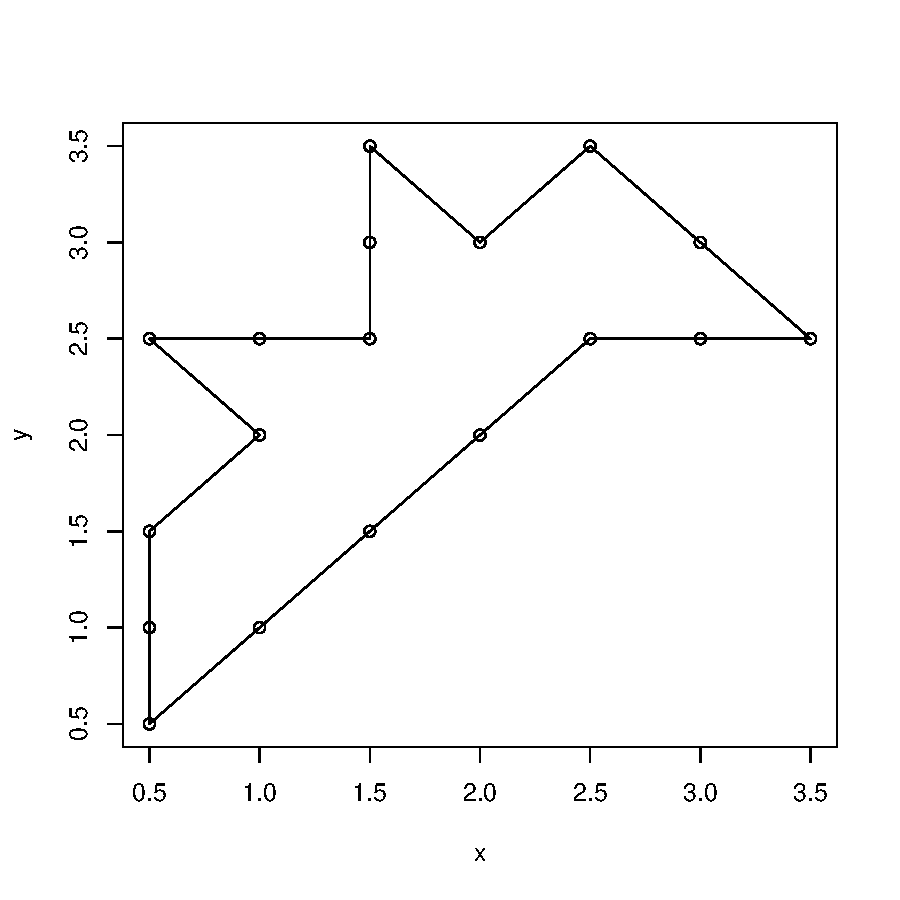
\includegraphics[scale=0.25]{fig/it4.pdf} \\
\includegraphics[scale=0.25]{fig/it8.pdf} &
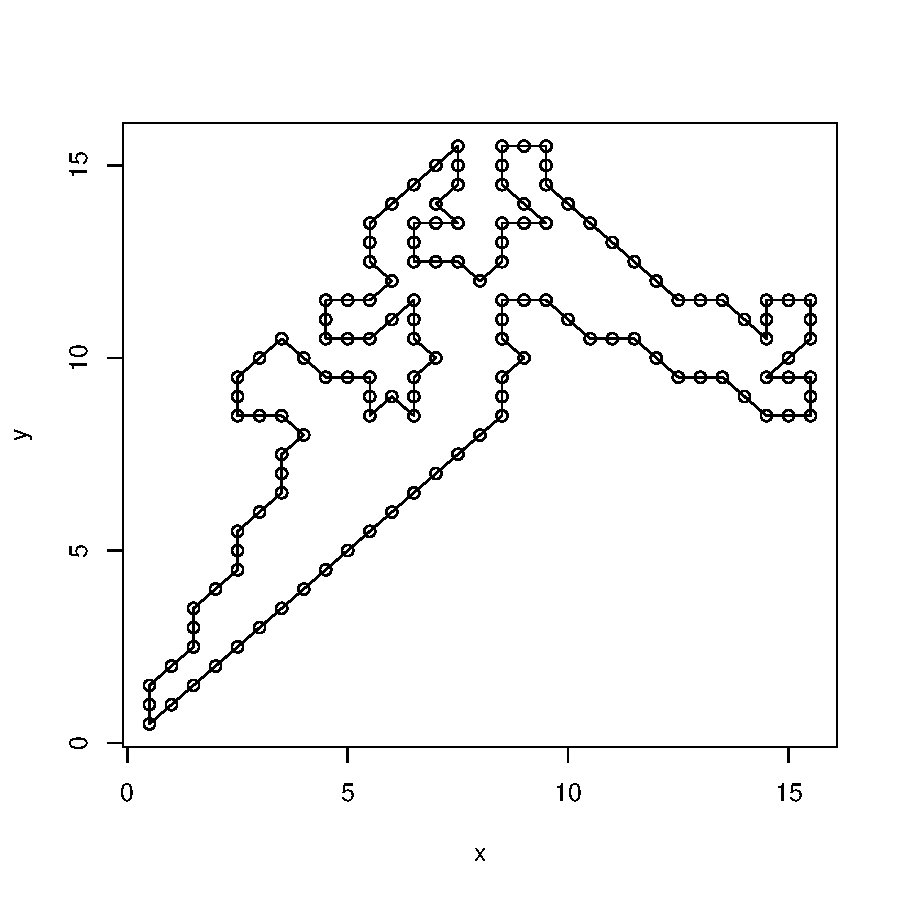
\includegraphics[scale=0.25]{fig/it16.pdf}
\end{tabular}
\caption{The first four iterations on d198.tsp}
\label{fig:iterations}
\end{center}
\end{figure}
When the first iteration is finished we can use earlier blocks to calculate an approximation of the shortest tour at a smaller scale. We can divide all the blocks in four subblocks to study the problem at a smaller scale. Instead of iterating over all the subblocks in the image, which can be quite time consuming at a very small scale, only the blocks which very visited in the previous estimated shortest tour are used in the calculation.
\newline\newline\noindent
The information which is retrieved from the previous scale, are the crossing points of the previous optimal path through the block. This optimal path can be seen in the top right picture of figure \ref{fig:renormalization}.  These crossing points are at the places, where the edges of the path, pass the borders of one of the cells. This is illustrated in the bottom right picture of figure \ref{fig:renormalization}. These crossing points, precalculated during the preprocessing stage, are used as start and ending point in the subblock. The optimal path between the starting and endpoint is retrieved, and placed in the subblock. The subblock is now a block on its own again, and can be used in the next scale.
\subsection{Retrieving the estimate of the shortest tour}
These process, which looks like zooming in on our microscope, is repeated until we reach unity. Unity is defined as the case where each cell has at most one city in it. Now we can directly retrieve our estimation of the shortest path. In figure \ref{fig:iterations} the first four iterations of the algorithm on $d198.tsp$ is shown. What is clear from this picture is that the route is refined in each iteration, until it exactly maps on the estimation  of the shortest tour.
\subsection{Parallelization}
This algorithm can be extended for parallel execution. We did not perform this extension, but we have a suggestion of how to do this. The foundation for parallelism is in the observation that we decreasing to a smaller scale, we divide all the blocks into four subblocks independently. So if the code needs to be parallelized, you first use one process to go to a scale where you have enough blocks in the whole area, to distribute over all the available processes. These can use these blocks to recursively divide them into four subblocks until they reached unity. Then the separate process can retrieve his part of the route and return it. In this method we achieve a high degree of parallelism since no intervening communication is required until the separate processes have found out their results. 
\section{Simulated Annealing}

% vim:ft=tex:spell spelllang=en:autoindent

